% !TEX root = ../notes.tex

\section{Underlying Notions}
{\centering \textbf{We are going to adopt the convention that every map is continuous unless otherwise stated.}}\\

\noindent
We want to be able to talk about ways to transform some shapes into other shapes and think about them then being equal. We do this by considering an $I \in [0, 1]$ that we can paramaterise a function by. So if we have two curves $s : X \to X$ and $t : X \to X$, we can define some $f : X \times I \to X$ such that,
$$ \begin{cases}
  f_0(x) &= s(x) \\
  f_1(x) &= t(x)
\end{cases} $$

\begin{ndefi}[Deformation Retraction]
  A Deformation retraction of a space $X$ onto an $A \subset X$ is a family of maps, $f_t : X \to X$ $t \in I$, such that, $f_0 = \1$, $f_t(X) = A$ and $f_t | A = \1$ $\forall t$. The family $f_t$ should be continuous in the sense that the associated map $X \times I \to X$, $(x, t) \mapsto f_t(x)$ is continuous.
\end{ndefi}

\begin{ndefi}[Mapping Cylinder]
  A mapping cylinder, $M_f$, for a $f : X \to Y$ is the quotient space of the disjoint union $(X \times I)\coprod Y$, obtained by identifying each $(x, 1) \in X \times I$ with $f(x) \in Y$.
\end{ndefi}

A mapping cylinder deformation, of $f$, retracts to $Y$.\\

A deformation retraction $f_t : X \to X$ is just a special case of a homotopy, which is just simply any family of maps, $f_t : X \times I \to Y$, given by $F(x, t) = f_t (x)$ is continuous.

\begin{ndefi}[Homotopic]
  One says two maps are homotopic if there exists a homotopy $f_t$ connecting them and one writes $f_0 \hm f_1$
\end{ndefi}

\textbf{Retractions are the topological analogue of projection operators.}

\begin{ndefi}[Homotopy Relative]
  A homotopy $f_t : X \to Y$ whose restriction to a subspace $A \subset X$ is independent of $t$ is homotopy relative, written as homotopy rel.
\end{ndefi}


\begin{ndefi}[Homotopy Equivalence]
  A map $f : X \to Y$ is called a homotopy equivalence if there exists a $g : Y \to X$ such that $fg \hm \1$ and $gf \hm \1$.
\end{ndefi}

Moreover, we can now say that $X$ and $Y$ are homotopy equivalent or have the same homotopy type.

\begin{nlemma}
  Any two spaces $X$ and $Y$ are homotopy equivilent if there exists some other space $Z$ containing both $X$ and $Y$ are deformation retracts.
\end{nlemma}

\begin{ndefi}[Contractible]
  A space that has the homotopy type of a point is contractible.
\end{ndefi}

This amounts to the identity map of this space to be nullhomotopic, that is homotopic to a constant map.

\subsection{Cell Complexes}

To construct a cell complex, let us follow these rules,
\begin{enumerate}
  \item Start with a discrete set $X^0$, whose points are regarded as $0$-cells.
  \item inductively, form the $n$-skeleton $X^n$ from $X^{n-1}$ by attaching $n$-cells $e^n_\a$ via maps $\phi_\a : S^{n-1} \to X^{n-1}$ with a collection of $n$-disks $D^n_\a$ under the identifications $x \sim \phi_\a (x)$ for $x \in \partial D^n_\a$. Thus $X^n = X^{n-1}\coprod_\a e^n_\a$.
  \item We can either stop at a finite amount or continue indefinitely. in the latter, $X$ is given a weak topology, A set $A \subset X$ is open if and only if $A \cap X^n$ is open in $X^n$ for each $n$. This similarly works for closed.
\end{enumerate}

$X$ is a cell complex or a CW complex. If $X = X^n$ then $X$ is said to be finite dimensional and the smallest such $n$ is the dimension of $X$, the maximum dimension of cells of $X$.

\begin{notation}
  $e^n$ denotes an $n$-cell.
\end{notation}

\begin{ndefi}[Characteristic Map]
  Each cell $e^n_\a$ in a cell complex $X$ has a characteristic map $\Phi_\a : D^n_\a \to X$ which extends $\phi_\a$ and is a homeomorphism from the interior of $D^n_\a$ onto $e^n_\a$. Namely, we can take $\phi_\a$ to be the composition, $D^n_\a \emd X^{n-1} \coprod_\a D^n_\a X^n \emd X^n$, where the middle map is the quotient map defining $X^n$.
\end{ndefi}

\begin{ndefi}[Subcomplex]
  A subcomplex of a cell complex $X$ is a closed subspace $A \subset X$ this is a union of cells of $X$.
\end{ndefi}

\begin{ndefi}[CW Pair]
  A complex $X$ with a subcomplex $A$, $(X, A)$, is called a CW pair.
\end{ndefi}

\subsection{Operations}
\begin{itemize}
  \item \textbf{Products:} We can take the product of two spaces, by just considering the product of the cells.
  \item \textbf{Quotients:} We can take quotients, of a CW pair $(X, A)$, by just quotienting out ($X \setminus A$) and adding the 0-cell, which acts as the image of $A$.
  \begin{intu}
    A quotient is just taking the $A$ space and moving it to a point. For example, let $X = D^2$ and $A = \partial D^2$, then, $X \setminus A \cong S^2$
    \begin{figure}[!ht]
    \centering
    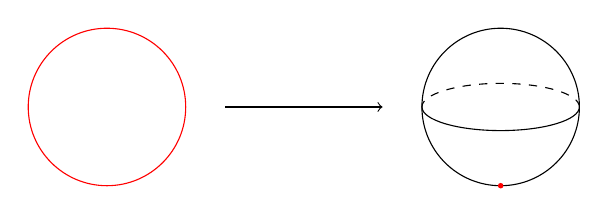
\begin{tikzpicture}
      \draw[red] (0,0) circle (1);
      \draw[->] (1.5, 0) -- (3.5,0);
      \draw (5,0) circle (1);
      \draw (4,0) arc (180:360:1 and 0.3);
      \draw[dashed] (6,0) arc (0:180:1 and 0.3);
      \fill[fill=red] (5,-1) circle (1pt);
    \end{tikzpicture}
    \caption{$X \sm A \cong S^2$}
    \end{figure}
  \end{intu}
  \item \textbf{Suspension: }Suspension is obtained by turning a space $X$ into a cylinder by considering $X \times I$ and then collapsing $X \times \{0\}$ and $X \times \{1\}$ to a point. We denote the suspension of a space by $SX$ and a cone by $CX$, both of these are CW complexes if $X$ is a CW complex.
  \item \textbf{Joins: }More generally we can talk about joins, this is where we consider the space $X \times Y \times I$, then instead of collapsing to a point, we collapse to a space. So we collapse $X \times Y \times \{0\}$ to $X$ and $X \times Y \times \{1\}$ to $Y$. This creates line segments. We can a join as $X * Y$. Then we can write each line segment as a formal linear combination of $a_1x+ a_2y$, where we say $a_1, a_2 \in [0,\,1]$ and $a_1 + a_2 = 1$, subject to $0x + 1y = y$ and $1x + 0y = x$. This can be generalised to many different spaces. One interesting example is when every $X_i$ is a single point. This leads to some thing called a simplex. If every point is a standard basis vector for $\R^n$, we get their join as the $(n-1)$-diensional simplex.
  \item \textbf{Wedge sum: }This is quite simple, this is just a single point union. We glue two spaces together at a single point. For example, taking $S^1 \v S^1$ and then getting a figure of eight after a wedge sum. More formally $X \v Y$ is the quotient of the disjoint union $X \coprod Y$ obtained by identitying a $x_0 \in X$ and $y_0 \in Y$ to a single point. Interestingly, for any cell complex $X$, the quotient $X^n \sm X^{n-1}$ is just a wedge sum of $n$-spheres $\V_\a S^n_\a$, with one sphere for each $n$-cell of $X$.
  \item \textbf{Smash Product: }This is slightly more complicated and will be used later. This is taking the points that we found with the wedge sum and just quotienting from the product space. So if we have $X$ and $Y$, our smash product is, $X \n Y = X \times Y \sm X \v Y$. An amusing and satifying fact is that $S^m \n S^n = S^{m+n}$ as we know that $S^n$ only has two cells, of dimension $0$ and $n$. This then means that when we smash two together we get another $n$-sphere. An example of this is on the next page:
  \begin{figure}[!ht]
  \centering
  \begin{tikzpicture}
% Torus
\draw (0,0) ellipse (1 and .75);
\begin{scope}
  \clip (0,-.9) ellipse (1 and 1.25);
  \draw(0,1.1) ellipse (1 and 1.25);
  \clip (0,1.1) ellipse (1 and 1.25);
  \draw (0,-1.1) ellipse (1 and 1.25);
  \fill[white] (7.5,-1.1) ellipse (1 and 1.25);
\end{scope}
\draw[red] (0,0) ellipse (0.8 and .47);
\draw[red] (0,.47) node[scale=0.8] {$<$};
\node (a) at (0.11,-.142894){};
\node (b) at (0.5,-.649519){};
\node (c) at ($(a)!0.5!(b)$) {};
\begin{scope}[shift={(c)},x={(a)}, scale=0.7]
\draw[red] (1,0) arc (0:180:1 and 0.3);
\draw[dashed, red] (-1,0) arc (180:360:1 and 0.3);
\end{scope}
\draw[red] (0.442,-0.555) node[scale=0.8,rotate=-85] {$<$};
\draw (0.17,-0.60);
\draw[->] (2, 0) -- (5, 0);
%% Sphere
\draw (7,0) circle (1);
\draw (6,0) arc (180:360:1 and 0.3);
\draw[dashed] (8,0) arc (0:180:1 and 0.3);
\fill[fill=red] (8,0) circle (1pt);
\end{tikzpicture}
  \caption{$S^1 \n S^1 \cong S^2$}
  \end{figure}
\end{itemize}

\subsection{Two Criteria for Homotopy Equivilence}
\subsubsection{Collapsing Subspaces}
\begin{claim}
  If $(X, A)$ are a CW pair consisting of a CW complex $X$ and a contractible subcomplex $A$, then the quotient map $X \to X \sm A$ is a homotopy equivilence.
\end{claim}
Then we can show that two spaces are homotopically equivilent by showing that through some quotienting and wedge sums the spaces are the same. For example, we can take a torus, then add four meridional discs, then transform it to three spheres, grab a line from a point between four of those discs and make `beads on a string', and finally we can make a bouquet by just pulling on the spheres a bit.

\subsection{Attaching Spaces}
We can attach one space to another without changing the homotopy type. This can be done with some mappings and image magic.\\

\noindent
Let us take two spaces $X_0$ and $X_1$ that we wish to attach. Now take $A \sub X_1$ and identify them with points in $X_0$. We now need the data of an map, $f : A \to X_0$, and form a quotient space of $X_0 \coprod X_1$ by identifying each $a \in A$ with its image $f(a) \in X_0$. Let us denote this space as $X_0 \sqcup_f X_1$, the space $X_0$ with $X_1$ attached along $A$ via $f$.\\

\noindent
The Mapping Cylinder $M_f$ is an example of this construction and we can consider a mapping cone $C_f = M_f \sm X$.

\begin{claim}
  If $(X, A)$ is a CW pair and the two attaching maps $f, g : A \to X_0$ are homotopic, then, $X_0 \sqcup_f X_1 \hm X_0 \sqcup X_1$.
\end{claim}

\subsection{Homotopy Extension Properties}
Consider the following, suppose we had a map $f_0 : X \to Y$ on a subspace $A \sub X$ and one is given a homotopy $f_t : A \to Y$ of $f_0 | A$ that one would like to extend to $f_t : X \to Y$ of the given $f_0$. If a pair $(X, A)$ is such a pair that this can always be solved we say that this pair has the homotopy extension property.

\begin{claim}
  A pair, $(X, A)$ has the homotopy extension property if and only if $X \times \{0\} \cup A \times I$ is a retract of $X \times I$.
\end{claim}

\begin{nprop}
  If $(X, A)$ is a CW pair, then $X \times \{0\} \cup A \times I$ is a defirmation retract of $X \times I$, hence $(X, A)$ has the homotopy extention property.
\end{nprop}
\begin{proof}
  Notice that $r : D^n \times I \to D^n \times \{0\} \times \partial D^n \times I$ is a retraction and then use that and the fact that you can just form $X$ and $A$ by attaching copies of $D^n \times I$ to $D^n \times \{0\} \times \partial D^n \times I$. Then preform a deformation retraction during $[\frac{1}{2^{n+1}},\, \frac{1}{2^n}]$.
\end{proof}

\begin{nprop}
  If the pair $(X, A)$ satisfies the homotopy extension property and $A$ is constractible, then the quotient map $q : X \to X \sm A$ is a homotopy equivilence.
\end{nprop}

\begin{minipage}[t]{0.4\textwidth}
\centering
  \[\begin{tikzcd}[ampersand replacement=\&]
  	X \&\& X \\
  	\\
  	{X\setminus A} \&\& {X\setminus A}
  	\arrow["{f_t}", from=1-1, to=1-3]
  	\arrow["q"', from=1-1, to=3-1]
  	\arrow["q", from=1-3, to=3-3]
  	\arrow["{\overline{f_t}}"', from=3-1, to=3-3]
  \end{tikzcd}\]
\end{minipage}
\begin{minipage}[t]{0.4\textwidth}
\centering
  \[\begin{tikzcd}[ampersand replacement=\&]
  	X \&\& X \\
  	\\
  	{X\setminus A} \&\& {X\setminus A}
  	\arrow["{f_1}", from=1-1, to=1-3]
  	\arrow["q"', from=1-1, to=3-1]
  	\arrow["q", from=1-3, to=3-3]
  	\arrow["{\overline{f_1}}"', from=3-1, to=3-3]
  	\arrow["g", from=3-1, to=1-3]
  \end{tikzcd}\]
\end{minipage}

\begin{proof}
  Let $f_t : X \to X$ be a homotopy extending contraction and then we can consider $f_0 = \1$ and then $qf_t : X \to X\sm A$ sending $A$ to a point and hence factors as a composition; $\begin{tikzcd}
	X & {X\setminus A} & {X\setminus A}
	\arrow["q", from=1-1, to=1-2]
	\arrow[from=1-2, to=1-3]
\end{tikzcd}$. Denoting the later map by $\overline{f_t} : X \sm A \to X \sm A$, we have that $qf_t = \overline{f_t}q$ as in the first diagram above. From here we consider a $g$ and a $q$ and prove homotopy equivalence.
\end{proof}

\begin{nprop}
  If $(X_1, A)$ is a CW pair and we have attaching maps $f, g : A \to X_0$ that are homotopic, then $X_0 \sqcup_f X_1 \hm X_0 \sqcup_g X_1 \rel X_0$
\end{nprop}

\begin{proof}
  Consider $F : A \times I \to X_0$ a homotopy from $f$ to $g$. Now consider $X_0 \sqcup (X_1 \times I)$, then this must contain $X_0 \sqcup_f X_1$ and $X_0 \sqcup_g X_1$ hence using Prop 0.14 we can prove this with a bit of fiddling with homotopies.
\end{proof}

\begin{nprop}
  Suppose that $(X, A)$ and $(Y, A)$ satisfy the homotopy extention property, and $f : X \to Y$ is a homotopy equivilence with $f | A = \1$. Then $f$ is a homotopy equivilence $\rel A$.
\end{nprop}

\begin{ncor}
 If $(X, A)$ satisfies the homotopy extension property and the inclusion $A \emd X$ is a homotopy equivilence, then $A$ is a deformation retract of $A$.
\end{ncor}

\begin{proof}
  Apply the proposition to the inclusion $A \emd X$.
\end{proof}

\begin{ncor}
 A map $f : X \to Y$ is a homotopy equivilence if and only if $X$ is a deformation retract of the mapping cylinder $M_f$. Hence, two spaces $X$ and $Y$ are homotopy equivilence $\rel A$. 
\end{ncor}
